\section{曲率与局部模型}
\label{sec:opt-smooth-local-models}

梯度方法用一个统一的$L$代替所有方向的曲率，预条件和动量只是在不知道真实曲率时的补救。若能读取二阶导数，就可以在当前点用二次模型~\eqref{eq:opt-smooth-quadratic-model}更贴切地代替目标，取$\bm B$为真实或近似的Hessian。这样做会遇到四个问题，本节按它们组织：曲率从哪里来（Hessian、修正后的Hessian，或由梯度差拼出的近似）；怎样保证模型可用（正定化、限制位移、加立方项）；怎样求解模型（直接分解或只用矩阵向量积的迭代）；以及怎样决定是否接受模型给出的位移（线搜索或比较实际与预测的下降）。贯穿始终的一点是：模型的最小点只是候选，原目标的检验不能省略；模型在局部最优，也不意味着原非凸目标已经全局最优。本节记$\bm g=\nabla f(\bm x)$，$\bm H=\nabla^2 f(\bm x)$；Hessian在某区域内的Lipschitz常数记为$M$，即$\lVert\nabla^2f(\bm u)-\nabla^2f(\bm v)\rVert_2\leq M\lVert\bm u-\bm v\rVert_2$。

\subsection{牛顿法}
\label{sec:opt-smooth-newton}

\paragraph{牛顿方程}
多元Taylor展开在$\bm x$附近给出二次模型
\[
  m(\bm p)=f(\bm x)+\langle\bm g,\bm p\rangle+\frac12\bm p^\top\bm H\bm p,
\]
其二阶余项的控制可参考\BookChapterRef{chap:multivariate-calculus}{卷一“多元函数微分”章}。令模型的梯度$\bm g+\bm H\bm p$为零，得到\term{牛顿法}（Newton's method）的方程与更新
\begin{equation}
\label{eq:opt-smooth-newton}
  \bm H\bm p^{\mathrm N}=-\bm g,\qquad \bm x^+=\bm x+\eta\,\bm p^{\mathrm N}.
\end{equation}
实际计算解这个线性方程，而不显式求$\bm H^{-1}$：$\bm H$正定时用Cholesky分解，稠密情形约需$d^3/3$次乘加和$O(d^2)$存储；求逆不但更贵，数值上也更不稳定。线性方程的直接解法及其误差分析可参考\BookChapterRef{chap:linear-equations-and-optimization}{卷一“线性方程与矩阵方程”章}。

\paragraph{可逆与正定的不同作用}
$\bm H$可逆只保证方程有唯一解，也就是模型有唯一驻点；$\bm H$正定才使这个驻点是模型的唯一最小点，并且$\langle\bm g,\bm p^{\mathrm N}\rangle=-\bm g^\top\bm H^{-1}\bm g<0$，即牛顿方向是下降方向。$\bm H$不定时，牛顿方向可能指向上坡。取$f(\bm x)=\tfrac12x_1^2+\tfrac14x_2^4-\tfrac12x_2^2$，它在$(0,\pm1)$处取最小值，原点是鞍点。在$\bm x=(0,0.2)^\top$处，$\bm g=(0,-0.192)^\top$，$\bm H=\operatorname{diag}(1,-0.88)$可逆但不定，牛顿方向$\bm p^{\mathrm N}=(0,-0.218)^\top$满足$\langle\bm g,\bm p^{\mathrm N}\rangle\approx0.042>0$。沿它走一整步到达$(0,-0.018)^\top$，目标从$-0.0196$升到约$-0.0002$，迭代被拉向鞍点。原因是二次模型在$x_2$方向开口向下，它的驻点是模型的最大点。

\paragraph{阻尼牛顿法}
远离最小点时，即使$\bm H$正定，二次模型也可能很不准确，整步会越过头。\term{阻尼牛顿法}（damped Newton method）保持牛顿方向不变，从$\eta=1$开始回溯，直到满足方向形式的Armijo条件
\[
  f(\bm x+\eta\bm p^{\mathrm N})\leq f(\bm x)+c\,\eta\langle\bm g,\bm p^{\mathrm N}\rangle,\qquad 0<c<\tfrac12 .
\]
它要求$\bm p^{\mathrm N}$是下降方向；对上坡方向，把步长缩得再小也只会使目标上升。单位步长必须最先试探且合格即接受，这一点在解附近至关重要：若永久固定$\eta<1$，在二次目标上误差每步只乘以$1-\eta$，快速局部收敛就丧失了。

\paragraph{局部二次收敛}
在非退化最小点附近，牛顿法以惊人的速度收敛。

\begin{theorem}[牛顿法的局部二次收敛]
\label{thm:opt-smooth-newton-local}
设$f$在球$\mathcal B=\{\bm x:\lVert\bm x-\bm x^\star\rVert_2<r\}$上二阶连续可微，$\nabla f(\bm x^\star)=\bm0$，并且在$\mathcal B$上$\nabla^2f\succeq\mu\bm I$（$\mu>0$）、Hessian是$M$-Lipschitz的。若$\bm x\in\mathcal B$，则单位牛顿步$\bm x^+=\bm x-\nabla^2f(\bm x)^{-1}\nabla f(\bm x)$满足
\begin{equation}
\label{eq:opt-smooth-newton-quadratic}
  \lVert\bm x^+-\bm x^\star\rVert_2\leq\frac{M}{2\mu}\lVert\bm x-\bm x^\star\rVert_2^2 .
\end{equation}
因此若$\lVert\bm x^{(0)}-\bm x^\star\rVert_2<\min\{r,2\mu/M\}$，全部迭代留在$\mathcal B$中，且$\tfrac{M}{2\mu}\lVert\bm x^{(t)}-\bm x^\star\rVert_2\leq\bigl(\tfrac{M}{2\mu}\lVert\bm x^{(0)}-\bm x^\star\rVert_2\bigr)^{2^t}$。
\end{theorem}

\begin{proof}
记$\bm e=\bm x-\bm x^\star$，$\bm H=\nabla^2f(\bm x)$。由于$\nabla f(\bm x^\star)=\bm0$，沿线段积分得$\nabla f(\bm x)=\int_0^1\nabla^2f(\bm x^\star+s\bm e)\bm e\,\mathrm ds$，于是
\[
  \bm x^+-\bm x^\star=\bm e-\bm H^{-1}\nabla f(\bm x)=\bm H^{-1}\int_0^1\bigl(\bm H-\nabla^2f(\bm x^\star+s\bm e)\bigr)\bm e\,\mathrm ds .
\]
$\lVert\bm H^{-1}\rVert_2\leq1/\mu$，被积项的范数不超过$M(1-s)\lVert\bm e\rVert_2^2$，积分得$\tfrac M2\lVert\bm e\rVert_2^2$，即式~\eqref{eq:opt-smooth-newton-quadratic}。若$\tfrac M{2\mu}\lVert\bm e\rVert_2<1$，则$\lVert\bm x^+-\bm x^\star\rVert_2<\lVert\bm e\rVert_2$，新点仍在$\mathcal B$中；记$a_t=\tfrac M{2\mu}\lVert\bm x^{(t)}-\bm x^\star\rVert_2$，式~\eqref{eq:opt-smooth-newton-quadratic}即$a_{t+1}\leq a_t^2$，归纳即得结论。
\end{proof}

误差满足$\lVert\bm e^{(t+1)}\rVert\leq C\lVert\bm e^{(t)}\rVert^2$的收敛称为\term{二次收敛}（quadratic convergence）：进入$a_t<1$的区域后，每步有效数字大约翻倍。图~\ref{fig:opt-smooth-newton-model}用一维例子$f(x)=e^x-2x$展示这一点，其最小点$x^\star=\ln2\approx0.6931$。从$x^{(0)}=1.5$出发，牛顿更新为$x^+=x-1+2e^{-x}$，误差依次约为$0.81$、$0.25$、$0.029$、$4.3\times10^{-4}$、$9.3\times10^{-8}$、$4.3\times10^{-15}$；比值$|e^{(t+1)}|/|e^{(t)}|^2$趋于$f'''(x^\star)/(2f''(x^\star))=1/2$。同一区间上$f''\leq e^{1.5}$，步长$e^{-1.5}$的梯度下降误差每步大约只乘以$1-2e^{-1.5}\approx0.55$。

\begin{figure}[htbp]
  \centering
  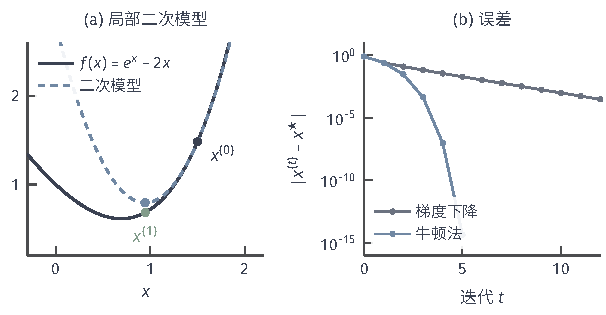
\includegraphics[width=102.6mm]{figures/03-optimization-evolution-and-signals/01-optimization/tikz/c3-newton-model/figure.pdf}
  \caption{牛顿法在$f(x)=e^x-2x$上的局部模型与误差。(a) 在$x^{(0)}=1.5$处的二阶Taylor模型（蓝色虚线）；它的最小点$x^{(1)}\approx0.946$就是牛顿步，模型值（蓝点）约$0.795$，真实目标（绿点）约$0.684$。(b) 误差$|x^{(t)}-\ln2|$的对数坐标：牛顿法（蓝）的曲线越来越陡，五步达到$10^{-15}$；步长$e^{-1.5}$的梯度下降（灰）是一条斜率固定的直线。}
  \label{fig:opt-smooth-newton-model}
\end{figure}

\paragraph{局部收敛阶与全程成本}
定理~\ref{thm:opt-smooth-newton-local}只描述已经进入半径$\min\{r,2\mu/M\}$的邻域之后的行为，这个邻域的大小在实际问题中通常未知。从远处出发时，阻尼牛顿法的线搜索阶段可能需要许多步，每步都要形成Hessian并分解，代价是$O(d^3)$；局部二次收敛只说明最后几步极快，不说明总成本低。两件事分开评价：局部收敛阶回答“到了附近以后误差怎样缩小”，全程成本回答“从初值到达给定精度一共做了多少工作”。第~\ref{sec:opt-smooth-accuracy-cost}节在共同标准下比较两者。

\subsection{修正牛顿法}
\label{sec:opt-smooth-modified-newton}

\paragraph{构造正定模型}
上一小节的例子说明，Hessian不定时牛顿方向可能上坡，而缩短步长无法补救：若$\langle\bm g,\bm p\rangle>0$，则对任意$\eta>0$都有$\langle\bm g,\eta\bm p\rangle>0$。补救必须改变方向本身。\term{修正牛顿法}（modified Newton method）把模型矩阵换成正定的$\bm B=\bm H+\bm E$，再解$\bm B\bm p=-\bm g$。最简单的修正是谱移位$\bm E=\delta\bm I$，取$\delta>\max\{0,-\lambda_{\min}(\bm H)\}$；不想计算特征值时，\term{修正Cholesky分解}（modified Cholesky factorization）在分解过程中遇到过小或负的主元就把它增大，同时得到某个正定的$\bm B$及其分解。在上一小节的点$(0,0.2)^\top$处取$\delta=1.88$，$\bm B=\operatorname{diag}(2.88,1)$，方向变为$(0,0.192)^\top$，沿它走一整步到$(0,0.392)^\top$，目标从$-0.0196$降到约$-0.071$，迭代离开鞍点、朝最小点$(0,1)$前进。

修正改变的是本轮用来求位移的模型，不改变原目标。所以修正后的位移仍要用原目标核验，例如对修正方向作Armijo回溯；修正矩阵正定只保证方向下降，不保证整步合格。

\paragraph{修正误差与求解残差}
修正牛顿与下一小节的不精确求解会同时引入误差，二者来源不同，应分别记录。设在第$t$轮用正定的$\bm B^{(t)}=\bm H^{(t)}+\bm E^{(t)}$求位移，线性方程只近似求解，残差为$\bm r^{(t)}=\bm B^{(t)}\bm p^{(t)}+\bm g^{(t)}$。在定理~\ref{thm:opt-smooth-newton-local}的邻域内，记$\bm e^{(t)}=\bm x^{(t)}-\bm x^\star$，与该定理的证明同样计算可得
\[
  \bm e^{(t+1)}=\bigl(\bm B^{(t)}\bigr)^{-1}\Bigl[\int_0^1\bigl(\bm H^{(t)}-\nabla^2f(\bm x^\star+s\bm e^{(t)})\bigr)\bm e^{(t)}\,\mathrm ds+\bm E^{(t)}\bm e^{(t)}+\bm r^{(t)}\Bigr].
\]
三项分别是模型的Taylor误差、曲率修正误差和方程求解残差。若$\lVert(\bm B^{(t)})^{-1}\rVert_2$一致有界，第一项给出二次项$O(\lVert\bm e^{(t)}\rVert^2)$；修正项给出$\lVert\bm E^{(t)}\rVert\lVert\bm e^{(t)}\rVert$，只有$\bm E^{(t)}\to\bm0$时才不拖累局部速度，$\lVert\bm E^{(t)}\rVert=O(\lVert\bm e^{(t)}\rVert)$或修正在有限步后为零时保持二次收敛。实际算法因此只在Hessian不正定时修正，进入Hessian正定的区域后令修正消失。

\paragraph{阻尼不是正则化}
永久保持$\bm E^{(t)}=\delta\bm I$的做法，只是让每一步的位移变短、方向偏向负梯度，最小点不变，但局部收敛退化为线性，误差因子约为$\delta/(\lambda+\delta)$。把原目标改成$f(\bm x)+\tfrac\delta2\lVert\bm x\rVert_2^2$是另一回事：它改变了问题和最小点，属于正则化，其作用在第~\ref{chap:opt-function-fitting}章讨论。两种操作在某一步的方程里看起来相似，含义完全不同。

\subsection{信赖域方法}
\label{sec:opt-smooth-trust-region}

修正牛顿法改变模型的曲率；另一种思路保留模型，限制位移的长度：模型只在当前点附近可信，那就只在附近找它的最小点，并根据模型预测得准不准来调整“附近”的范围。

\paragraph{子问题与候选步}
\term{信赖域}（trust region）方法在第$t$轮求解
\begin{equation}
\label{eq:opt-smooth-trust-subproblem}
  \min_{\bm p}\ m(\bm p)=f(\bm x)+\langle\bm g,\bm p\rangle+\frac12\bm p^\top\bm B\bm p\qquad\text{满足}\ \lVert\bm p\rVert_2\leq\Delta ,
\end{equation}
其中$\bm B$可以是Hessian或其近似，允许不定；半径$\Delta>0$限制的是本轮位移，原问题仍然无约束。子问题不必精确求解，常用三种候选步。\term{Cauchy点}（Cauchy point）沿$-\bm g$在球内最小化模型：$\bm g^\top\bm B\bm g\leq0$时走到边界，否则取$\bm p^{\mathrm C}=-\tau\bm g$，$\tau=\min\{\lVert\bm g\rVert_2^2/(\bm g^\top\bm B\bm g),\ \Delta/\lVert\bm g\rVert_2\}$。它只用一次矩阵向量积，是衡量其他候选步的基准。\term{狗腿法}（dogleg method）要求$\bm B\succ\bm0$：沿折线从原点到无约束的Cauchy点$\bm p^{\mathrm U}=-(\lVert\bm g\rVert_2^2/\bm g^\top\bm B\bm g)\bm g$，再到牛顿点$\bm p^{\mathrm B}=-\bm B^{-1}\bm g$，取折线与球面的交点（牛顿点在球内时直接取它）。模型值沿这条折线单调下降，所以交点给出比Cauchy点更好的模型值。第三种是下一小节的截断共轭梯度法，适合$\bm B$很大或不定的情形。

\paragraph{比较实际与预测的下降}
候选步$\bm p$求出后，用\term{下降比}（reduction ratio）衡量模型预测得准不准：
\begin{equation}
\label{eq:opt-smooth-trust-ratio}
  \rho=\frac{f(\bm x)-f(\bm x+\bm p)}{m(\bm0)-m(\bm p)} .
\end{equation}
分母是模型预测的下降，分子是实际下降。$\rho$接近$1$说明模型在这个半径内可信，可以放大半径；$\rho$很小或为负说明模型在这个距离上已不可信。

\begin{algorithm}[信赖域方法的一轮]
\label{alg:opt-smooth-trust-region}
\begin{algorithmic}[1]
\Require 当前点$\bm x$，$\bm g$，模型矩阵$\bm B$，半径$\Delta$，上限$\Delta_{\max}$，接受阈值$\eta_{\mathrm a}\in[0,1/4)$
\Ensure 下一点与新半径
\State 近似求解子问题~\eqref{eq:opt-smooth-trust-subproblem}得$\bm p$，要求预测下降$m(\bm0)-m(\bm p)>0$
\State 计算$f(\bm x+\bm p)$与$\rho$
\If{$\rho<1/4$} \State $\Delta\gets\Delta/4$
\ElsIf{$\rho>3/4$ 且 $\lVert\bm p\rVert_2=\Delta$} \State $\Delta\gets\min\{2\Delta,\Delta_{\max}\}$
\EndIf
\If{$\rho>\eta_{\mathrm a}$} \State \Return $\bm x+\bm p$与新的$\Delta$ \Comment{接受}
\Else \State \Return $\bm x$与新的$\Delta$ \Comment{拒绝，下一轮在同一点用缩小的半径重求}
\EndIf
\end{algorithmic}
\end{algorithm}

拒绝不浪费梯度和Hessian：下一轮在同一点、用同一模型、以更小的半径重解子问题，只多花一次函数值计算和一次子问题求解。若预测下降不为正，比值没有意义。$\bm g\neq\bm0$时Cauchy点的预测下降严格为正，所以这种情况说明子问题求解出了错，应检查内层；若$\bm g=\bm0$且$\bm B\succeq\bm0$，模型在原点已经最小，算法应按驻点停止，并另行判断曲率（见第~\ref{sec:opt-smooth-nonconvex}节）。

\begin{example}[一次拒绝与一次接受]
\label{ex:opt-smooth-trust-region}
取$f(x)=x^4/4$，在$x=1$处$g=1$。假设所用曲率近似为$B=1/2$（真实二阶导数是$3$，这个近似严重偏小），模型$m(p)=\tfrac14+p+\tfrac14p^2$的无约束最小点在$p=-2$。第一次取$\Delta=2$，候选步$p=-2$到达$x=-1$，预测下降$m(0)-m(-2)=1$，实际下降$f(1)-f(-1)=0$，$\rho=0$，拒绝并把半径缩为$1/2$。第二次候选步在边界上，$p=-1/2$，到达$x=1/2$，预测下降$1/2-1/16=7/16$，实际下降$1/4-1/64=15/64$，$\rho=15/28\approx0.54$，接受，半径保持$1/2$。图~\ref{fig:opt-smooth-trust-region}(b)画出了这两次试探。
\end{example}

图~\ref{fig:opt-smooth-trust-region}(a)在共同例上画出狗腿法。在$\bm x=(2,2)^\top$处，无约束的Cauchy点为$\bm p^{\mathrm U}\approx(-0.125,-2.007)^\top$，长度约$2.01$；牛顿点$\bm p^{\mathrm B}=(-2,-2)^\top$，长度约$2.83$。取$\Delta=2.5$，折线在第二段上与球面相交，得$\bm p\approx(-1.497,-2.002)^\top$，新点约为$(0.503,-0.002)^\top$。模型就是目标本身，所以$\rho=1$，预测下降约$33.87$，比Cauchy点的$32.24$更多。

\begin{figure*}[htbp]
  \centering
  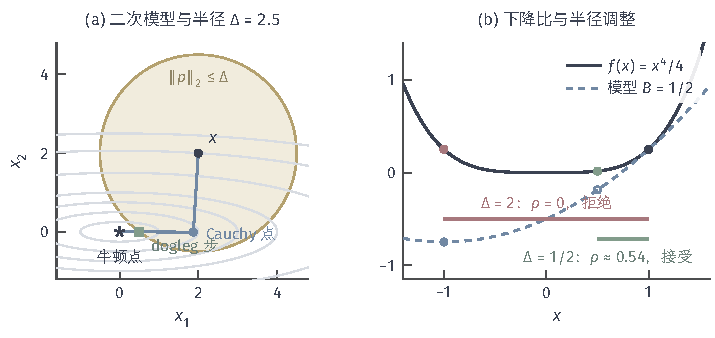
\includegraphics[width=121.1mm]{figures/03-optimization-evolution-and-signals/01-optimization/tikz/c3-trust-region/figure.pdf}
  \caption{信赖域方法。(a) 共同例在$\bm x=(2,2)^\top$处的二次模型等高线与半径$\Delta=2.5$的信赖域（黄色圆盘）。蓝色折线从$\bm x$到Cauchy点，再到位于域外的牛顿点（原点）；绿色方块是折线与边界的交点，即狗腿步。(b) 例~\ref{ex:opt-smooth-trust-region}：$f(x)=x^4/4$与$x=1$处曲率偏小的模型（$B=1/2$）。红色线段是$\Delta=2$的信赖区间，模型最小点$x=-1$处的真实目标（红点）并不低于出发点，$\rho=0$；绿色线段是缩小后的$\Delta=1/2$，候选点$x=1/2$被接受。空心点是模型在候选点的值。}
  \label{fig:opt-smooth-trust-region}
\end{figure*}

\paragraph{收敛条件}
信赖域方法的全局收敛论证需要几项条件同时成立：每轮候选步的预测下降至少是Cauchy点预测下降的固定比例，即$m(\bm0)-m(\bm p)\geq c_1\lVert\bm g\rVert_2\min\{\Delta,\lVert\bm g\rVert_2/\lVert\bm B\rVert_2\}$；模型矩阵一致有界；目标下有界且梯度在相关水平集附近Lipschitz连续；接受规则如算法~\ref{alg:opt-smooth-trust-region}。在这些条件下可以证明$\liminf_{t\to\infty}\lVert\nabla f(\bm x^{(t)})\rVert_2=0$，取$\eta_{\mathrm a}>0$时还有$\lim_{t\to\infty}\lVert\nabla f(\bm x^{(t)})\rVert_2=0$\cite{math-nocedal2006numerical}。论证的骨架是：半径足够小时模型误差相对预测下降可忽略，$\rho$接近$1$，所以半径不会无限缩小；而每次接受都使目标下降一个与梯度相关的量，目标有下界，梯度就不能一直很大。只说“子问题在球内被精确最小化”不能代替这些条件，而模型在球内的全局最小点，也不是原非凸目标的全局最小点。

\subsection{不精确牛顿与Newton--CG}
\label{sec:opt-smooth-newton-cg}

当$d$达到数万乃至更大时，形成并分解$d\times d$的Hessian都不可行。但很多问题可以廉价地计算\term{Hessian向量积}（Hessian-vector product）$\bm v\mapsto\nabla^2f(\bm x)\bm v$：由$\nabla^2f(\bm x)\bm v=\lim_{h\to0}(\nabla f(\bm x+h\bm v)-\nabla f(\bm x))/h$可以用两次梯度差分近似，自动微分则能以常数倍于一次梯度的代价精确计算它。只用这种乘积近似求解牛顿方程的方法，称为\term{不精确牛顿法}（inexact Newton method）；内层用共轭梯度法时称为\term{Newton--CG法}（Newton--CG method）。

\paragraph{内层：截断共轭梯度}
共轭梯度法（CG）在系数矩阵对称正定时求解线性方程，每步一次矩阵向量积，算法与收敛性可参考上文引用的卷一“线性方程与矩阵方程”章。用于$\bm H\bm p=-\bm g$时，$\bm H$可能不定，所以需要在每步检查方向上的曲率；同时规定方程残差$\bm r=\bm H\bm p+\bm g$小到什么程度就停止。

\begin{algorithm}[Newton--CG的内层（线搜索版本）]
\label{alg:opt-smooth-newton-cg}
\begin{algorithmic}[1]
\Require Hessian向量积$\bm v\mapsto\bm H\bm v$，梯度$\bm g\neq\bm0$，精度参数$\vartheta\in(0,1)$
\Ensure 候选方向$\bm p$与停止原因
\State $\bm p_0\gets\bm0$，$\bm r_0\gets\bm g$，$\bm d_0\gets-\bm g$
\For{$j=0,1,2,\dots$}
  \State $\kappa_j\gets\bm d_j^\top\bm H\bm d_j$
  \If{$\kappa_j\leq0$} \State \Return $\bm p_j$（$j=0$时返回$-\bm g$），原因：非正曲率 \EndIf
  \State $a_j\gets\lVert\bm r_j\rVert_2^2/\kappa_j$，$\bm p_{j+1}\gets\bm p_j+a_j\bm d_j$，$\bm r_{j+1}\gets\bm r_j+a_j\bm H\bm d_j$
  \If{$\lVert\bm r_{j+1}\rVert_2\leq\vartheta\lVert\bm g\rVert_2$} \State \Return $\bm p_{j+1}$，原因：残差达标 \EndIf
  \State $b_j\gets\lVert\bm r_{j+1}\rVert_2^2/\lVert\bm r_j\rVert_2^2$，$\bm d_{j+1}\gets-\bm r_{j+1}+b_j\bm d_j$
\EndFor
\end{algorithmic}
\end{algorithm}

算法只在曲率为正时才用它的倒数计算步长，所以每个已接受的内步都使模型下降，返回的$\bm p$是下降方向。外层仍对$\bm p$作Armijo回溯，用原目标决定接受。信赖域版本（Steihaug的截断CG）作两处改动：遇到非正曲率时沿$\bm d_j$走到信赖域边界，新位移越出边界时截在边界上，再交给算法~\ref{alg:opt-smooth-trust-region}按下降比判断。于是内层有三种停止原因：残差达标、遇到非正曲率、触及信赖域边界。实现中应分别记录，因为它们说明不同的情况：第一种说明方程解得够准，后两种说明模型在当前范围内不适合求其驻点。

\paragraph{精度控制与局部收敛阶}
内层解得多准，决定外层能保持多快的局部速度。用随外层变化的参数$\vartheta^{(t)}$规定$\lVert\bm r^{(t)}\rVert_2\leq\vartheta^{(t)}\lVert\bm g^{(t)}\rVert_2$，序列$(\vartheta^{(t)})$称为\term{强迫序列}（forcing sequence）。在定理~\ref{thm:opt-smooth-newton-local}的邻域内（$\nabla^2f\succeq\mu\bm I$，Hessian为$M$-Lipschitz），设$\vartheta^{(t)}\leq\bar\vartheta<1$且接受单位步。由$\bm p=(\bm H^{(t)})^{-1}(-\bm g^{(t)}+\bm r^{(t)})$得$\lVert\bm p\rVert_2\leq(1+\bar\vartheta)\lVert\bm g^{(t)}\rVert_2/\mu\leq2\lVert\bm g^{(t)}\rVert_2/\mu$。新梯度为
\[
  \begin{aligned}
  \bm g^{(t+1)}&=\bm g^{(t)}+\bm H^{(t)}\bm p+\int_0^1\bigl(\nabla^2f(\bm x^{(t)}+s\bm p)-\bm H^{(t)}\bigr)\bm p\,\mathrm ds\\
  &=\bm r^{(t)}+\int_0^1\bigl(\nabla^2f(\bm x^{(t)}+s\bm p)-\bm H^{(t)}\bigr)\bm p\,\mathrm ds ,
  \end{aligned}
\]
取范数得
\begin{equation}
\label{eq:opt-smooth-inexact-newton}
  \lVert\bm g^{(t+1)}\rVert_2\leq\vartheta^{(t)}\lVert\bm g^{(t)}\rVert_2+\frac M2\lVert\bm p\rVert_2^2\leq\Bigl(\vartheta^{(t)}+\frac{2M}{\mu^2}\lVert\bm g^{(t)}\rVert_2\Bigr)\lVert\bm g^{(t)}\rVert_2 .
\end{equation}
括号中的因子说明了三种情形。$\vartheta^{(t)}\leq\bar\vartheta<1$固定时，梯度足够小后因子小于某个$q<1$，梯度范数线性收敛；$\vartheta^{(t)}\to0$时因子趋于零，即\term{超线性收敛}（superlinear convergence）；$\vartheta^{(t)}\leq C\lVert\bm g^{(t)}\rVert_2$时右边是$\lVert\bm g^{(t)}\rVert_2^2$的倍数，恢复二次收敛。这里保证的是梯度范数的收敛阶；在该邻域内$\mu\lVert\bm x-\bm x^\star\rVert_2\leq\lVert\nabla f(\bm x)\rVert_2$，参数误差随之受控。固定内层CG步数并不对应某个确定的$\vartheta$，因为同样步数达到的残差还取决于谱分布与预条件。

\paragraph{内层工作与外层收益}
$\vartheta^{(t)}$越小，内层CG步越多，每步一次Hessian向量积。远离解时二次模型本身就不准确，把模型方程解到很高精度只增加成本，不能改善原目标的下降，所以常见的选择是让$\vartheta^{(t)}$随$\lVert\bm g^{(t)}\rVert_2$一起减小，例如$\vartheta^{(t)}=\min\{1/2,\sqrt{\lVert\bm g^{(t)}\rVert_2}\}$，它在远处宽松、在近处给出超线性收敛。每轮存储只需几个$d$维向量，这是Newton--CG相对于完整牛顿法的主要优势。

\paragraph{CG看不到的方向}
CG只在Krylov子空间$\operatorname{span}\{\bm g,\bm H\bm g,\bm H^2\bm g,\dots\}$中工作，它没有遇到负曲率，不说明$\bm H$半正定。取$\bm H=\operatorname{diag}(1,-1)$，$\bm g=(1,0)^\top$：$\bm H\bm g=\bm g$，Krylov子空间就是$x_1$轴，CG第一步得到$\kappa_0=1>0$、$\bm p_1=(-1,0)^\top$，残差为零，正常结束，完全看不到$x_2$方向的曲率$-1$。所以Newton--CG的“残差达标”不能当作二阶最优性的证据；需要认证没有负曲率时，必须用第~\ref{sec:opt-smooth-nonconvex}节的曲率检测。

\subsection{拟牛顿方法}
\label{sec:opt-smooth-quasi-newton}

Hessian向量积仍要求能对梯度再求导。若只有梯度可用，能否从迭代过程中已经算出的梯度里“拼出”曲率？

\paragraph{割线条件}
走完一步后，我们知道位移和梯度的变化：
\[
  \bm s^{(t)}=\bm x^{(t+1)}-\bm x^{(t)},\qquad\bm y^{(t)}=\nabla f(\bm x^{(t+1)})-\nabla f(\bm x^{(t)}),
\]
由沿线段积分，$\bm y^{(t)}$又可写成
\[
  \bm y^{(t)}=\Bigl(\int_0^1\nabla^2f(\bm x^{(t)}+\tau\bm s^{(t)})\,\mathrm d\tau\Bigr)\bm s^{(t)} .
\]
$\bm y^{(t)}$记录了沿$\bm s^{(t)}$方向的平均曲率作用；对二次目标恰有$\bm y=\bm H\bm s$。\term{拟牛顿法}（quasi-Newton method）要求新的模型矩阵复现这一观测，即\term{割线条件}（secant condition）
\begin{equation}
\label{eq:opt-smooth-secant}
  \bm B^{(t+1)}\bm s^{(t)}=\bm y^{(t)} .
\end{equation}
一维时它唯一确定$B^{(t+1)}=y/s$，正是导数曲线上两点连线的斜率。图~\ref{fig:opt-smooth-secant}(a)取$f(x)=e^x-2x$，$x^{(t)}=0$、$x^{(t+1)}=1$：割线斜率$e-1\approx1.718$介于两端的真实曲率$1$与$e\approx2.718$之间。$d>1$时，割线条件只给出$d$个方程，对称矩阵却有$d(d+1)/2$个自由度，还需要一条规则决定其余部分。

\paragraph{BFGS更新}
BFGS更新\cite{math-nocedal2006numerical}在满足割线条件的前提下，只用两个秩一修正改动旧矩阵：
\begin{equation}
\label{eq:opt-smooth-bfgs}
  \bm B^{(t+1)}=\bm B^{(t)}+\frac{\bm y\bm y^\top}{\bm y^\top\bm s}-\frac{\bm B^{(t)}\bm s\bm s^\top\bm B^{(t)}}{\bm s^\top\bm B^{(t)}\bm s},
\end{equation}
这里省略了$\bm s,\bm y$的上标。直接验证：$\bm B^{(t+1)}\bm s=\bm B^{(t)}\bm s+\bm y-\bm B^{(t)}\bm s=\bm y$。对与$\bm s$正交（在$\bm B^{(t)}$内积下）的方向，第三项不起作用，第二项的作用也只沿$\bm y$，所以更新在“已经观测过的方向”上记住新曲率，其余方向基本保留旧的估计。

\begin{example}[一次BFGS更新保留了什么]
\label{ex:opt-smooth-bfgs}
在共同例上取$\bm B^{(0)}=\bm I$。若位移$\bm s=(0,1)^\top$，则$\bm y=\bm H\bm s=(0,16)^\top$，更新给出$\bm B^{(1)}=\bm I+\operatorname{diag}(0,16)-\operatorname{diag}(0,1)=\operatorname{diag}(1,16)$，一步就得到真实Hessian，因为$\bm s$恰是特征方向。若位移$\bm s=(1,1)^\top$，则$\bm y=(1,16)^\top$，$\bm y^\top\bm s=17$，$\bm s^\top\bm B^{(0)}\bm s=2$，
\[
  \bm B^{(1)}=\bm I+\frac1{17}\begin{pmatrix}1&16\\16&256\end{pmatrix}-\frac12\begin{pmatrix}1&1\\1&1\end{pmatrix}=\frac1{34}\begin{pmatrix}19&15\\15&529\end{pmatrix}.
\]
可以核对$\bm B^{(1)}\bm s=(1,16)^\top=\bm y$。沿$\bm s$它与$\bm H$完全一致，沿与之正交的$(1,-1)^\top$，二次型$\bm v^\top\bm B^{(1)}\bm v=518/34\approx15.2$，而真实值是$17$，只是部分地学到了。图~\ref{fig:opt-smooth-secant}(b)把三个矩阵画成椭圆$\bm v^\top\bm M\bm v=1$：$\bm B^{(1)}$的椭圆与$\bm H$的椭圆恰好在$\pm\bm s/\sqrt{17}$处相交。
\end{example}

\begin{figure}[htbp]
  \centering
  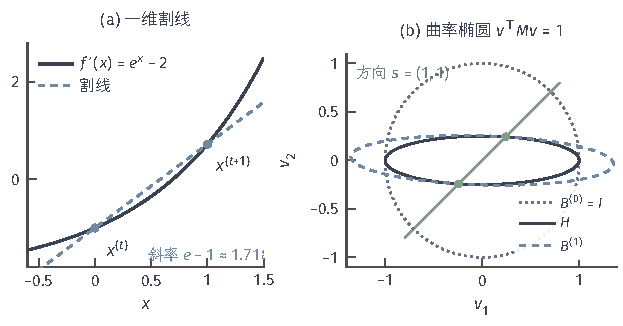
\includegraphics[width=105.5mm]{figures/03-optimization-evolution-and-signals/01-optimization/tikz/c3-secant/figure.pdf}
  \caption{割线条件怎样拼出曲率。(a) $f'(x)=e^x-2$在$x^{(t)}=0$与$x^{(t+1)}=1$两点的割线（蓝色虚线），斜率$e-1$是这段区间上的平均曲率。(b) 例~\ref{ex:opt-smooth-bfgs}中三个矩阵$\bm M$的曲率椭圆$\bm v^\top\bm M\bm v=1$：灰色点线为初始$\bm B^{(0)}=\bm I$，黑色为真实$\bm H=\operatorname{diag}(1,16)$，蓝色虚线为沿$\bm s=(1,1)^\top$更新一次后的$\bm B^{(1)}$。绿色直线是$\bm s$方向，$\bm B^{(1)}$与$\bm H$的椭圆在绿点处重合。}
  \label{fig:opt-smooth-secant}
\end{figure}

\paragraph{曲率条件与线搜索}
BFGS更新保持正定的关键是\term{曲率条件}（curvature condition）$\bm y^\top\bm s>0$。设$\bm B^{(t)}\succ\bm0$且$\bm y^\top\bm s>0$，对任意$\bm v\neq\bm0$，由$\bm B^{(t)}$内积的Cauchy--Schwarz不等式，$\bm v^\top\bm B^{(t)}\bm v-(\bm s^\top\bm B^{(t)}\bm v)^2/(\bm s^\top\bm B^{(t)}\bm s)\geq0$，等号仅在$\bm v$与$\bm s$平行时成立，而此时$(\bm y^\top\bm v)^2/(\bm y^\top\bm s)>0$；两部分相加即$\bm v^\top\bm B^{(t+1)}\bm v>0$。强凸目标总满足曲率条件；一般目标上，线搜索要额外保证它。只缩短步长的Armijo回溯做不到这一点，需要再加上\term{Wolfe曲率条件}（Wolfe curvature condition）
\[
  \nabla f(\bm x+\eta\bm p)^\top\bm p\geq c_2\,\nabla f(\bm x)^\top\bm p,\qquad 0<c<c_2<1,
\]
它排除了步长过短、斜率还很陡的点。满足它时$\bm y^\top\bm s=\eta\bigl(\nabla f(\bm x+\eta\bm p)-\nabla f(\bm x)\bigr)^\top\bm p\geq\eta(c_2-1)\nabla f(\bm x)^\top\bm p>0$。若某一步观测到的曲率不可靠，实现中可以跳过该次更新或对$\bm y$作阻尼修正。

\paragraph{逆近似与L-BFGS}
实际计算中维护逆近似$\bm C=\bm B^{-1}$更方便，方向为$-\bm C\bm g$，由Sherman--Morrison--Woodbury公式，式~\eqref{eq:opt-smooth-bfgs}等价于
\[
  \bm C^{(t+1)}=\bigl(\bm I-\omega\bm s\bm y^\top\bigr)\bm C^{(t)}\bigl(\bm I-\omega\bm y\bm s^\top\bigr)+\omega\bm s\bm s^\top,\qquad\omega=\frac1{\bm y^\top\bm s}.
\]
每轮$O(d^2)$运算和$O(d^2)$存储，不需要解线性方程。$d$很大时连$d^2$也存不下。\term{有限内存拟牛顿法}（limited-memory BFGS，L-BFGS）只保存最近$r$对$(\bm s_i,\bm y_i)$，从一个简单的初始逆近似$\bm C_0$（常取$\gamma\bm I$，$\gamma=\bm s^\top\bm y/\bm y^\top\bm y$取自最近一对）出发，隐式地施加这$r$次更新，用两次循环直接算出方向$\bm C\bm g$，而不形成矩阵。

\begin{algorithm}[L-BFGS的双循环递推]
\label{alg:opt-smooth-lbfgs}
\begin{algorithmic}[1]
\Require 梯度$\bm g$，最近$r$对$(\bm s_i,\bm y_i)$（$i=k-r,\dots,k-1$，均满足$\bm y_i^\top\bm s_i>0$），初始尺度$\gamma>0$
\Ensure $\bm z=\bm C\bm g$，方向取$-\bm z$
\State $\bm q\gets\bm g$
\For{$i=k-1,k-2,\dots,k-r$} \Comment{从新到旧}
  \State $\omega_i\gets1/(\bm y_i^\top\bm s_i)$，$\alpha_i\gets\omega_i\bm s_i^\top\bm q$，$\bm q\gets\bm q-\alpha_i\bm y_i$
\EndFor
\State $\bm z\gets\gamma\bm q$
\For{$i=k-r,\dots,k-1$} \Comment{从旧到新}
  \State $b\gets\omega_i\bm y_i^\top\bm z$，$\bm z\gets\bm z+(\alpha_i-b)\bm s_i$
\EndFor
\end{algorithmic}
\end{algorithm}

每轮约$4rd$次乘加，存储$2rd$个数；$r$常取$5$到$20$。完整BFGS在$\bm x^\star$处Hessian正定、Hessian在邻域内Lipschitz、单位步优先尝试且合格即接受等条件下，局部超线性收敛；其证明依赖$\bm B^{(t)}$沿实际位移方向逐渐逼近真实Hessian\cite{math-nocedal2006numerical}。L-BFGS不断丢弃旧信息，这一逼近一般不成立，完整BFGS的超线性结论不能直接移用；它的实际效果通常很好，但理论保证要按有限记忆的形式另行说明。另一个常被提到的性质，“正定二次目标上用精确线搜索的BFGS至多$d$步终止”，也只在精确线搜索这一特殊条件下成立。

\subsection{立方正则化（补充）}
\label{sec:opt-smooth-cubic}

信赖域用硬半径限制位移；本小节介绍一种用光滑的惩罚限制位移的模型，它把Hessian的Lipschitz常数直接写进模型，因而在非凸目标上也能给出清楚的下降量与复杂度。初读可以跳过，第~\ref{sec:opt-smooth-nonconvex}节只用到其中的结论。

\paragraph{三阶余项与立方模型}
若Hessian在包含线段$[\bm x,\bm x+\bm p]$的凸区域上$M$-Lipschitz，与下降引理同样沿线段积分两次，得
\[
  f(\bm x+\bm p)\leq f(\bm x)+\langle\bm g,\bm p\rangle+\frac12\bm p^\top\bm H\bm p+\frac M6\lVert\bm p\rVert_2^3 .
\]
\term{立方正则化}（cubic regularization）的牛顿法\cite{nesterov2006cubic}在第$t$轮最小化
\begin{equation}
\label{eq:opt-smooth-cubic-model}
  m_\sigma(\bm p)=f(\bm x)+\langle\bm g,\bm p\rangle+\frac12\bm p^\top\bm H\bm p+\frac\sigma3\lVert\bm p\rVert_2^3,\qquad\sigma>0 .
\end{equation}
取$\sigma\geq M/2$时，$m_\sigma$是$f(\bm x+\bm p)$的上界，模型下降就保证实际下降，这是下降引理在二阶上的对应物。立方项在远处的增长快过二次项，即使$\bm H$不定，模型也有全局最小点；它惩罚的是本轮位移，不改变原目标。图~\ref{fig:opt-smooth-cubic-model}取$f(x)=x^4/4-x^2/2$，在$x=0.2$处$g=-0.192$、$H=-0.88$，二次模型开口向下、没有最小点；区间$[-1,1]$上$|f'''|\leq6$，取$\sigma=3$，立方模型的最小点为$s\approx0.439$，到达$x+s\approx0.639$，目标从$-0.0196$降到约$-0.163$。

\begin{figure}[htbp]
  \centering
  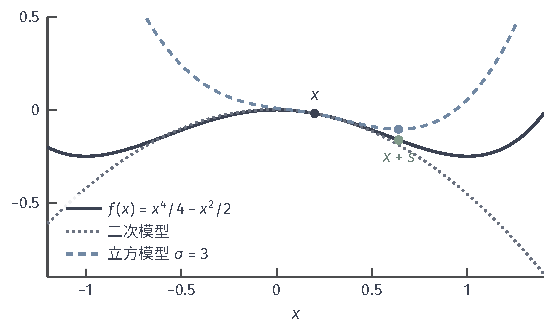
\includegraphics[width=92.9mm]{figures/03-optimization-evolution-and-signals/01-optimization/tikz/c3-cubic-model/figure.pdf}
  \caption{$f(x)=x^4/4-x^2/2$（黑）在$x=0.2$处的局部模型。二次模型（灰色点线）的曲率$-0.88$为负，向两侧无界下降；加上$\tfrac\sigma3|p|^3$（$\sigma=3$）后的立方模型（蓝色虚线）在区间$[-1,1]$上位于$f$之上，最小点给出$s\approx0.439$。蓝点是模型值约$-0.104$，绿点是真实目标约$-0.163$。}
  \label{fig:opt-smooth-cubic-model}
\end{figure}

\paragraph{模型最小点的刻画}
可以证明，$\bm s$是$m_\sigma$的全局最小点，当且仅当下面两式同时成立\cite{nesterov2006cubic}：
\[
  \bm g+\bm H\bm s+\sigma\lVert\bm s\rVert_2\bm s=\bm0,\qquad\bm H+\sigma\lVert\bm s\rVert_2\bm I\succeq\bm0 .
\]
第一式是模型的驻点方程，第二式是附加的曲率条件；只满足第一式的点可能是模型的鞍点或局部最大点，所以近似求解时只看模型梯度小不够。图中$H+\sigma s=-0.88+3\times0.439\approx0.44\geq0$，两式都成立。

\paragraph{下降量与新点的梯度}
设$\sigma\geq M/2$，$\bm s$满足上面两式。由驻点方程，$\langle\bm g,\bm s\rangle=-\bm s^\top\bm H\bm s-\sigma\lVert\bm s\rVert_2^3$，代入模型得
\[
  \begin{aligned}
  m_\sigma(\bm s)-f(\bm x)&=-\frac12\bm s^\top\bm H\bm s-\frac{2\sigma}3\lVert\bm s\rVert_2^3\\
  &\leq\frac\sigma2\lVert\bm s\rVert_2^3-\frac{2\sigma}3\lVert\bm s\rVert_2^3=-\frac\sigma6\lVert\bm s\rVert_2^3,
  \end{aligned}
\]
其中用了曲率条件给出的$\bm s^\top\bm H\bm s\geq-\sigma\lVert\bm s\rVert_2^3$。所以$f(\bm x)-f(\bm x+\bm s)\geq\tfrac\sigma6\lVert\bm s\rVert_2^3$。另一方面，新点的梯度
\[
  \begin{aligned}
  \nabla f(\bm x+\bm s)&=\bm g+\bm H\bm s+\int_0^1\bigl(\nabla^2f(\bm x+\tau\bm s)-\bm H\bigr)\bm s\,\mathrm d\tau\\
  &=-\sigma\lVert\bm s\rVert_2\bm s+\int_0^1\bigl(\nabla^2f(\bm x+\tau\bm s)-\bm H\bigr)\bm s\,\mathrm d\tau,
  \end{aligned}
\]
故$\lVert\nabla f(\bm x+\bm s)\rVert_2\leq(\sigma+M/2)\lVert\bm s\rVert_2^2$。把两式连起来：只要新点的梯度范数大于$\varepsilon$，本步的下降就至少为$\tfrac\sigma6\bigl(\varepsilon/(\sigma+M/2)\bigr)^{3/2}$。若$f$下有界，这样的步至多有$O(\varepsilon^{-3/2})$个，于是在$O(\varepsilon^{-3/2})$轮内得到$\lVert\nabla f\rVert_2\leq\varepsilon$的点；梯度下降的对应界是$O(\varepsilon^{-2})$（定理~\ref{thm:opt-smooth-gd-nonconvex}）。

\paragraph{这个复杂度计了什么}
$O(\varepsilon^{-3/2})$数的是外层轮数，也就是目标、梯度与Hessian的求值次数。每轮的子问题本身需要求解，精确求解通常要特征分解或解一个一维非线性方程，代价可达$O(d^3)$。用近似子问题解代替时，近似解必须同时达到上面用到的模型下降、驻点方程残差和曲率条件的相应精度，复杂度结论才能保留。$M$未知时，实现中按与下降比~\eqref{eq:opt-smooth-trust-ratio}同样的方式根据接受结果调整$\sigma$。
